% IEEE-format PBL-2 project report (updated from report-writing-paper.docx, 16 October 2026)
% Course: SRM Report Writing (21CSC402P), Department of Computing Technologies
% Authors: Aditya Sahu (RA2311026010814), Akash Cherian (RA2311026010852), Prachurya Subhasmita (RA2311026010855)

\documentclass[conference]{IEEEtran}

\usepackage[T1]{fontenc}
\usepackage{amsmath,amssymb}
\usepackage{booktabs}
\usepackage{cite}
\usepackage{array}
\usepackage{url}
\usepackage{microtype}
\usepackage{hyperref}
\usepackage{balance}
\usepackage{tikz}
\usetikzlibrary{arrows.meta,positioning,fit,calc}

\def\UrlBreaks{\do\/\do-}

\hypersetup{
  colorlinks=true,
  linkcolor=black,
  citecolor=black,
  urlcolor=black
}

\title{Reliability-Aware Audio-Visual Fusion for Generalizable Deepfake Detection}

\author{
  \IEEEauthorblockN{Aditya Sahu}
  \IEEEauthorblockA{\textit{Dept. of Computing Technologies} \\
  \textit{SRM Institute of Science \& Technology} \\
  Kattankulathur, Chennai, India \\
  Reg. No.: RA2311026010814 \\
  as8962@srmist.edu.in}
  \and
  \IEEEauthorblockN{Akash Cherian}
  \IEEEauthorblockA{\textit{Dept. of Computing Technologies} \\
  \textit{SRM Institute of Science \& Technology} \\
  Kattankulathur, Chennai, India \\
  Reg. No.: RA2311026010852 \\
  ac7809@srmist.edu.in}
  \and
  \IEEEauthorblockN{Prachurya Subhasmita}
  \IEEEauthorblockA{\textit{Dept. of Computing Technologies} \\
  \textit{SRM Institute of Science \& Technology} \\
  Kattankulathur, Chennai, India \\
  Reg. No.: RA2311026010855 \\
  ps2200@srmist.edu.in}
}

\IEEEspecialpapernotice{(PBL-2 Project Report --- Course: 21CSC402P Report Writing, Assessment Date: 16 October 2026)}

\begin{document}
\maketitle

\begin{abstract}
This report documents the technology choices for a lightweight audio-visual deepfake detector and analyses the evidence available from its preliminary implementation. The stack uses Python and PyTorch, FFmpeg, OpenCV and torchaudio for media processing, a MobileNetV3-Small visual encoder, a depthwise-separable CNN audio encoder, and a small multilayer perceptron that estimates per-window modality weights. Reproducibility is supported by identity-grouped split manifests, YAML configuration, mixed-precision training targeted to a single 6--8~GB GPU, and a scikit-learn/SciPy evaluation layer. The reported data-pipeline audit partitions 21,544 local FakeAVCeleb clips into identity-disjoint training, validation and test sets of 15,018, 2,136 and 4,390 clips. A single-epoch validation snapshot records AUROC values of 0.7974 for visual-only, 0.8625 for audio-only, 0.9426 for equal-weight fusion and 0.7957 for reliability-aware fusion. These are preliminary validation-only observations: there are no test metrics, repeated-seed estimates, confidence intervals, calibration results or robustness results. The snapshot neither supports nor refutes the project hypotheses. We describe the diagnostics and staged experiments required for a defensible conclusion.
\end{abstract}

\begin{IEEEkeywords}
Audio-visual deepfake detection, multimodal fusion, reliability estimation, technology stack, preliminary evaluation, reproducibility.
\end{IEEEkeywords}

\section{Introduction}
Recent developments in generative artificial intelligence have substantially lowered the barrier to synthesizing photorealistic facial reenactments, identity swaps, and expressive text-to-speech or voice conversion. When deployed maliciously, multimodal deepfakes threaten digital trust, authentication systems, and legal evidence integrity. Although single-modality detectors targeting facial artifacts~\cite{haliassos2021} or synthetic acoustic spectral cues~\cite{liu2023asvspoof,tak2021rawnet2,jung2022aasist} have progressed, unimodal models fail when confronted with manipulations targeting the unmonitored modality (e.g., cloned audio accompanying authentic video, or face swaps paired with genuine speech)~\cite{khalid2021,muppalla2023}. 

Multimodal deepfake detection aims to resolve this vulnerability by jointly examining visual and acoustic streams. However, joint detectors face two fundamental challenges:
\begin{enumerate}
    \item \textbf{Asymmetric Modality Reliability:} Real-world media routinely encounters transmission artifacts, low lighting, motion blur, face detection failures, ambient acoustic noise, or codec compression. Under such asymmetric degradation, naive fusion strategies that treat both streams equally allow a severely corrupted modality to inject uninformative noise, diluting authentic forensic evidence~\cite{zhou2021,cai2025modality}.
    \item \textbf{Synchronization Ambiguity:} While desynchronization between speech and lip motion can reveal automated manipulation~\cite{chugh2020,chung2016}, genuine media frequently exhibits non-zero temporal offsets due to audio-video transmission latency, dubbing, or video editing. Conversely, state-of-the-art lip-sync generators (e.g., Wav2Lip) produce synthetic videos with near-perfect temporal alignment. Hence, synchronization mismatch must serve as an auxiliary feature, never as an independent authenticity verdict.
\end{enumerate}

Prior works have explored dynamic multimodal weighting; therefore, this work makes no claim of pioneering dynamic fusion concepts~\cite{wang2024}. Instead, this paper investigates a specific, lightweight architecture that calculates per-window reliability weights $(w_v, w_a)$ directly conditioned on transparent physical quality signals (blur variance, luminance, audio signal-to-noise ratio proxy, voice activity), unimodal prediction uncertainty, and normalized cross-correlation sync features. The primary research questions are:
\begin{itemize}\setlength{\itemsep}{1.5pt}\setlength{\parskip}{0pt}\setlength{\parsep}{0pt}
    \item \textbf{RQ1:} Does learned per-window reliability weighting improve AUROC, balanced accuracy, and calibration over unimodal and fixed-fusion baselines?
    \item \textbf{RQ2:} Under isolated audio or video degradation, does the gate shift its weights in the expected direction and reduce the performance drop?
    \item \textbf{RQ3:} On unseen manipulation categories, does the model match or exceed the strongest unimodal baseline?
    \item \textbf{RQ4:} Can a compact model achieve practical short-window latency with a documented accuracy cost?
\end{itemize}

\section{Related Work and Research Gap}

\subsection{Audio-Visual Synchronization and Forensic Inconsistency}
Early multimodal forensic investigations focused on detecting cross-modal dissonance. Chugh et al.~\cite{chugh2020} proposed a Modality Dissonance Score (MDS) leveraging 3D convolutional visual features and Mel-spectrogram audio embeddings to localize temporal tampering. Mittal et al.~\cite{mittal2020} developed a Siamese network comparing affective facial expressions with vocal prosody, identifying mismatches in emotional valence. Chung and Zisserman~\cite{chung2016} introduced SyncNet, training two-stream contrastive encoders to quantify lip-to-speech temporal synchronization. While pioneering, these frameworks assume that temporal desynchronization directly implies manipulation---an assumption that fails on authentic dubbed video or well-aligned modern deepfakes. LipForensics, introduced by Haliassos et al.~\cite{haliassos2021}, demonstrated that high-level spatio-temporal mouth motion dynamics generalize across unseen face manipulations, yet it operates as a unimodal visual model blind to synthetic speech.

\subsection{Multimodal Benchmarks and Heavyweight Architectures}
The release of FakeAVCeleb by Khalid et al.~\cite{khalid2021} and the DeepFake Detection Challenge (DFDC) dataset by Dolhansky et al.~\cite{dolhansky2020} provided important benchmarks for deepfake research. Recent methods explore cross-attention and masked feature learning~\cite{yang2023,oorloff2024}, transformer-based encoders~\cite{ilyas2023}, and statistical summaries across audio and video~\cite{astrid2024}. The present project chooses smaller components for a modest-GPU setting; its results are not equal-compute comparisons with these larger architectures.

\subsection{Multimodal Learning Dynamics and Reliability Gating}
In multimodal learning, branches can learn at different rates and compete during joint optimization. Wang, Tran, and Feiszli~\cite{wang2020gblend} analyzed this behavior and proposed Gradient Blending (G-Blend); Peng et al.~\cite{peng2022ogm} proposed On-the-Fly Gradient Modulation (OGM-GE) to adjust dominant modality gradients. Muppalla, Jia, and Lyu~\cite{muppalla2023} report that naive concatenation can underperform unimodal baselines on FakeAVCeleb. Wang et al.~\cite{wang2024} study dynamic audio-visual weighting from transformer prediction confidences. These works motivate fixed-fusion baselines and diagnostics for modality imbalance.

\subsection{Audio Anti-Spoofing and Missing Modalities}
Acoustic deepfake forensics has established that voice synthesis detectors are vulnerable to compression codecs and acoustic noise, as benchmarked extensively in the ASVspoof 2021 evaluation by Liu et al.~\cite{liu2023asvspoof}, AASIST by Jung et al.~\cite{jung2022aasist}, and RawNet2 by Tak et al.~\cite{tak2021rawnet2}. Furthermore, facial analysis literature demonstrates that input image degradation directly impacts feature reliability; Terh{\"o}rst et al.~\cite{terhorst2020serfiq} formalized this in SER-FIQ by linking stochastic embedding variance to face image quality. In the forensic domain, Cai et al.~\cite{cai2025modality} demonstrated that standard joint detectors collapse when an entire modality is missing (e.g., muted audio or occluded video), proposing an auxiliary AVSR pre-training approach to handle modality dropout.

\subsection{Research Gap and Proposed Scope}
Prior work motivates multimodal fusion, dynamic weighting, quality measures and cross-modal signals. This project implements a compact configuration-driven system with an inspectable gate conditioned on quality ($q_v,q_a$), unimodal uncertainty ($u_v,u_a$) and synchronization features ($c$), trained with a detached soft-target loss ($\mathcal{L}_{\mathrm{rel}}$). The intended evaluation uses source-identity-disjoint splits and controlled degradation and missing-modality conditions. This scope makes no claim of introducing dynamic fusion or of a measured robustness benefit before those experiments are complete.

\section{Problem Formulation}
Let a video clip be partitioned into short windows containing visual stream $V$ and acoustic stream $A$. Let $y \in \{0, 1\}$ represent the binary authenticity label ($y=0$ for genuine, $y=1$ for manipulated). Compact visual and audio encoders map inputs into temporal-bin feature sequences:
\begin{equation}
  z_v \in \mathbb{R}^{T \times D}, \qquad z_a \in \mathbb{R}^{T \times D},
\end{equation}
where $T=8$ temporal bins and $D=256$ feature channels. Mean-pooled embeddings are denoted $\bar{z}_v = \frac{1}{T}\sum_t z_{v,t}$ and $\bar{z}_a = \frac{1}{T}\sum_t z_{a,t}$.

Unimodal classification heads produce preliminary forensic probabilities $p_v = \sigma(\ell_v^{\mathrm{logit}})$ and $p_a = \sigma(\ell_a^{\mathrm{logit}})$, from which epistemic uncertainty proxies are extracted:
\begin{equation}
  u_m = 1 - 2|p_m - 0.5| \in [0, 1], \qquad m \in \{v, a\}.
\end{equation}

For each window, physical quality vectors $q_v \in \mathbb{R}^7$ and $q_a \in \mathbb{R}^5$ are computed alongside missingness flags $m_v, m_a \in \{0, 1\}$. Modality features are projected to a 128-D shared metric space via linear layers $\phi_v$ and $\phi_a$, from which auxiliary synchronization cross-correlation features $c \in \mathbb{R}^4$ are extracted across temporal offsets $\delta \in \{-2, -1, 0, 1, 2\}$.

Modality summary vectors are constructed as:
\begin{equation}
  h_v = [\bar{z}_v, \, q_v, \, m_v, \, u_v], \qquad h_a = [\bar{z}_a, \, q_a, \, m_a, \, u_a].
\end{equation}
The reliability estimator receives $[h_v, h_a, c]$ and generates gate logits $g = \mathrm{MLP}([h_v, h_a, c]) \in \mathbb{R}^2$. The final modality reliability weights are computed as:
\begin{equation}
  [w_v, w_a] = \operatorname{softmax}(g / T_g), \qquad w_v + w_a = 1,
\end{equation}
where $T_g$ is a temperature hyperparameter. The fused classification head $F$ predicts the final deepfake probability $p_f$:
\begin{equation}
  p_f = \sigma(F([w_v \bar{z}_v, \; w_a \bar{z}_a, \; c, \; w_v, \; w_a])).
\end{equation}
The weights $w_v$ and $w_a$ estimate forensic usefulness under the training distribution; they do not represent ground-truth physical quality or authenticity labels.

\section{Proposed System and Technologies}

\subsection{Input and Preprocessing Pipeline}
The input pipeline processes media clips at a standardized rate of 25 frames per second (fps). Each two-second analysis window samples 16 uniformly spaced face frames (effective 8 fps visual sampling rate) and 2.0 seconds of synchronized mono audio resampled to 16 kHz. 

\textbf{Visual Processing:} Facial regions are detected, expanded by a 20\% margin to retain jawline and forehead boundary artifacts, and resized to $160 \times 160$ RGB pixels. Seven recorded quality values are detection-success rate, Laplacian blur variance ($\sigma_{\mathrm{Lap}}^2$), face area, mean luminance, luminance standard deviation, mean saturation, and failed-frame fraction. A detector-confidence value may be retained as metadata but is not part of this seven-value vector. If face detection fails on more than 4 of 16 frames, the window is retained with visual missingness flag $m_v = 1$ and zeroed tensors, avoiding silent data dropouts.

\textbf{Audio Processing:} Acoustic streams are converted to 80-bin log-Mel spectrograms utilizing a 25-ms Hann window, 10-ms hop size, and 512-point FFT. Five acoustic quality values are extracted: VAD speech fraction, root-mean-square (RMS) energy, clipped-sample ratio, estimated SNR proxy, and duration mismatch. Muted or silent audio segments set $m_a = 1$.

\begin{figure*}[t]
\centering
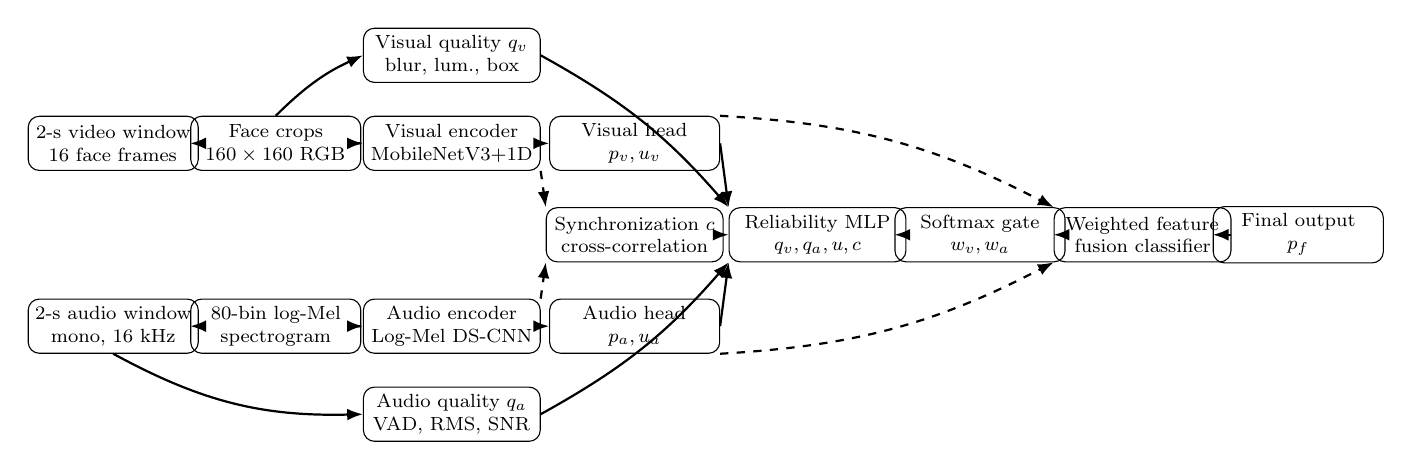
\begin{tikzpicture}[
  font=\footnotesize,
  scale=0.86,transform shape,
  box/.style={draw,rounded corners,align=center,minimum height=8mm,text width=23mm,inner sep=3pt},
  wide/.style={draw,rounded corners,align=center,minimum height=8mm,text width=24mm,inner sep=3pt},
  flow/.style={-{Latex[length=2mm]},thick},
  hint/.style={-{Latex[length=2mm]},thick,dashed}
]
% Row 1: Visual stream (y = 1.35) and Top Quality (y = 2.65)
\node[box] (video) at (0, 1.35) {2-s video window\\16 face frames};
\node[box] (face) at (2.4, 1.35) {Face crops\\$160\times160$ RGB};
\node[wide] (ve) at (5.0, 1.35) {Visual encoder\\MobileNetV3+1D};
\node[wide] (qualityv) at (5.0, 2.65) {Visual quality $q_v$\\blur, lum., box};
\node[box] (headv) at (7.7, 1.35) {Visual head\\$p_v, u_v$};

% Row 3: Audio stream (y = -1.35) and Bottom Quality (y = -2.65)
\node[box] (audio) at (0, -1.35) {2-s audio window\\mono, 16 kHz};
\node[box] (mel) at (2.4, -1.35) {80-bin log-Mel\\spectrogram};
\node[wide] (ae) at (5.0, -1.35) {Audio encoder\\Log-Mel DS-CNN};
\node[wide] (qualitya) at (5.0, -2.65) {Audio quality $q_a$\\VAD, RMS, SNR};
\node[box] (heada) at (7.7, -1.35) {Audio head\\$p_a, u_a$};

% Row 2: Central fusion pipeline (y = 0)
\node[wide] (sync) at (7.7, 0) {Synchronization $c$\\cross-correlation};
\node[wide] (gate) at (10.4, 0) {Reliability MLP\\$q_v, q_a, u, c$};
\node[box] (weight) at (12.8, 0) {Softmax gate\\$w_v, w_a$};
\node[wide] (fusion) at (15.2, 0) {Weighted feature\\fusion classifier};
\node[box] (out) at (17.5, 0) {Final output\\$p_f$};

% Flows for Visual stream
\draw[flow] (video) -- (face);
\draw[flow] (face) -- (ve);
\draw[flow] (face.north) to[bend left=10] (qualityv.west);
\draw[flow] (ve) -- (headv);
\draw[hint] (ve.south east) -- (sync.north west);

% Flows for Audio stream
\draw[flow] (audio) -- (mel);
\draw[flow] (mel) -- (ae);
\draw[flow] (audio.south) to[bend right=15] (qualitya.west);
\draw[flow] (ae) -- (heada);
\draw[hint] (ae.north east) -- (sync.south west);

% Converging inputs into Reliability MLP
\draw[flow] (qualityv.east) to[bend left=10] (gate.north west);
\draw[flow] (headv.east) -- (gate.north west);
\draw[flow] (sync.east) -- (gate.west);
\draw[flow] (heada.east) -- (gate.south west);
\draw[flow] (qualitya.east) to[bend right=10] (gate.south west);

% Gate to classifier to output
\draw[flow] (gate) -- (weight);
\draw[flow] (weight) -- (fusion);
\draw[flow] (fusion) -- (out);

% Feature bypass to fusion classifier
\draw[hint] (headv.north east) to[bend left=12] (fusion.north west);
\draw[hint] (heada.south east) to[bend right=12] (fusion.south west);
\end{tikzpicture}
\caption{End-to-end architecture of the proposed reliability-aware audio-visual deepfake detector. Quality signals ($q_v, q_a$), unimodal uncertainties ($u_v, u_a$), and cross-correlation synchronization ($c$) inform the gating MLP to dynamically weight visual and acoustic representations ($w_v, w_a$) prior to fusion classification.}
\label{fig:architecture}
\end{figure*}

\subsection{Architectural Sub-Modules}
The complete system (Fig.~\ref{fig:architecture}) comprises seven coordinated modules:
\begin{itemize}
    \item \textbf{Visual Encoder ($z_v$):} A MobileNetV3-Small convolutional backbone~\cite{howard2019}, with optional ImageNet-pretrained weights, processes individual face crops. The 16 frame embeddings are aggregated into $T=8$ temporal bins via a depthwise temporal Conv1D layer (kernel size 3, stride 2, padding 1), generating $z_v \in \mathbb{R}^{8 \times 256}$. The visual encoder parameter count remains to be measured.
    \item \textbf{Audio Encoder ($z_a$):} A 2D depthwise-separable convolutional neural network (DS-CNN, configurable width multiplier 0.75--1.0) processes the 80-bin log-Mel spectrogram. Five depthwise-separable blocks reduce spectrogram dimensions, followed by adaptive average pooling along the time axis to $T=8$ bins, producing $z_a \in \mathbb{R}^{8 \times 256}$.
    \item \textbf{Alignment Projector:} Separate linear projection heads map $z_v$ and $z_a$ into a shared 128-dimensional metric space: $\tilde{z}_{v,t} = W_{\mathrm{proj},v} z_{v,t}$ and $\tilde{z}_{a,t} = W_{\mathrm{proj},a} z_{a,t}$.
    \item \textbf{Synchronization Cross-Correlation Extractor ($c$):} For temporal offsets $\delta \in \{-2, -1, 0, 1, 2\}$, cosine similarities are computed across corresponding temporal bins:
    \begin{equation}
      s_\delta = \frac{1}{T - |\delta|} \sum_{t} \frac{\tilde{z}_{v,t} \cdot \tilde{z}_{a,t+\delta}}{\|\tilde{z}_{v,t}\|_2 \|\tilde{z}_{a,t+\delta}\|_2}.
    \end{equation}
    The four-dimensional synchronization vector $c = [s_0, \, \max_\delta s_\delta, \, \arg\max_\delta s_\delta, \, \operatorname{Var}(s_\delta)]$ summarizes temporal alignment, peak correspondence, optimal lag, and cross-offset dispersion.
    \item \textbf{Modality Classification Heads:} Linear layers map $\bar{z}_v$ and $\bar{z}_a$ to unimodal logits $\ell_v^{\mathrm{logit}}$ and $\ell_a^{\mathrm{logit}}$ for auxiliary supervision.
    \item \textbf{Reliability Estimator:} A 2-layer MLP (Linear $532 \to 128$, ReLU, Dropout 0.1, Linear $128 \to 2$) receives $[h_v,h_a,c]$ and outputs gate logits $g$. The 532-value implementation-derived input count differs from the roughly 30--50 feature estimate in the canonical project brief; this discrepancy should be reconciled before final experiments.
    \item \textbf{Weighted Fusion Classifier:} The fusion representation $f = [w_v \bar{z}_v, \, w_a \bar{z}_a, \, c, \, w_v, \, w_a] \in \mathbb{R}^{518}$ is passed through the repository classifier (Linear $518\to256$, ReLU, Dropout 0.2, Linear $256\to128$, ReLU, Dropout 0.2, Linear $128\to1$) to compute the final prediction logit. This differs from the $518\to256\to1$ topology stated in the new report document.
\end{itemize}

\subsection{Training Objectives and Detached Soft Target}
Let $\ell_v = \mathrm{BCE}(y, p_v)$ and $\ell_a = \mathrm{BCE}(y, p_a)$ denote the instantaneous per-window unimodal cross-entropy losses. To supervise the reliability gate without backpropagating gradients through the modality heads, a detached soft target is formulated:
\begin{equation}
  t_m = \frac{\exp(-\operatorname{stopgrad}(\ell_m)/\tau_r)}{\sum_{j \in \{v, a\}} \exp(-\operatorname{stopgrad}(\ell_j)/\tau_r)}, \quad m \in \{v, a\},
  \label{eq:soft_target}
\end{equation}
where $\tau_r > 0$ is a target temperature hyperparameter. The reliability regularization loss is defined as the Kullback--Leibler divergence between soft target $t$ and predicted weights $w$:
\begin{equation}
  \mathcal{L}_{\mathrm{rel}} = \mathrm{KL}(t \parallel w) = \sum_{m \in \{v, a\}} t_m \log\left(\frac{t_m}{w_m}\right).
  \label{eq:l_rel}
\end{equation}
The full multi-task objective combines fused classification, unimodal auxiliary regularization, reliability loss, and an optional gate entropy balance term:
\begin{equation}
  \mathcal{L} = \mathcal{L}_f + \alpha(\mathcal{L}_v + \mathcal{L}_a) + \beta \mathcal{L}_{\mathrm{rel}} + \gamma \mathcal{L}_{\mathrm{con}} + \eta \mathcal{L}_{\mathrm{bal}},
  \label{eq:total_loss}
\end{equation}
where $\mathcal{L}_f = \mathrm{BCE}(y, p_f)$, $\mathcal{L}_{\mathrm{con}}$ denotes optional InfoNCE contrastive alignment on genuine media pairs~\cite{oord2018}, and $\mathcal{L}_{\mathrm{bal}} = \sum_m (w_m - 0.5)^2$ is an optional penalty active only during warm-up to prevent premature single-modality collapse. Hyperparameters are configured as $\alpha = 0.25$, $\beta = 0.1$, $\gamma = 0.05$, $\eta = 0.0$, and $\tau_r = 1.0$.

\subsection{Implementation Technologies}
Table~\ref{tab:technologies} summarizes the technical stack, framework choices, and implementation status across all sub-components.

\begin{table}[t]
\caption{Implementation Technologies and Component Status}
\label{tab:technologies}
\centering
\scriptsize
\setlength{\tabcolsep}{3pt}
\renewcommand{\arraystretch}{1.15}
\begin{tabular}{>{\raggedright\arraybackslash}p{2.3cm}>{\raggedright\arraybackslash}p{5.8cm}}
\toprule
\textbf{Subsystem / Tool} & \textbf{Technical Role and Implementation Status} \\
\midrule
\textbf{Visual Encoder} & MobileNetV3-Small backbone~\cite{howard2019} (ImageNet pre-trained) with depthwise temporal Conv1D ($K=3$, $T=8$, $D=256$). \emph{Implemented}. \\
\textbf{Audio Encoder} & 80-bin log-Mel front-end (25\,ms window, 10\,ms hop) + 2D depthwise-separable CNN ($T=8$, $D=256$). \emph{Implemented}. \\
\textbf{Alignment \& Sync} & Linear projections to 128-D shared metric space; cross-correlation over offsets $\delta \in \{-2,\dots,+2\}$. \emph{Implemented}. \\
\textbf{Quality Extraction} & Face detection box ratio, Laplacian blur variance, luminance; audio RMS, clipping, SNR proxy, VAD. \emph{Implemented}. \\
\textbf{Reliability MLP} & 2-layer MLP ($532 \to 128 \to 2$, ReLU, dropout 0.1) yielding softmax gate weights $(w_v, w_a)$ at temperature $T_g$. \emph{Implemented}. \\
\textbf{Classifier Head} & Repository code: $518 \to 256 \to 128 \to 1$, dropout 0.2, over $[w_v \bar{z}_v,w_a \bar{z}_a,c,w_v,w_a]$. The DOCX states $518\to256\to1$. \emph{Topology discrepancy}. \\
\textbf{Execution Stack} & PyTorch 2.x~\cite{paszke2019}, torchaudio, torchvision, Automatic Mixed Precision~\cite{micikevicius2018}, gradient accumulation (effective batch 32). \emph{Implemented}. \\
\textbf{Media Decoding} & FFmpeg/ffprobe (25\,fps video, 16\,kHz mono audio), OpenCV Haar face detector~\cite{viola2001}. \emph{Implemented baseline}. \\
\textbf{Data \& Config} & NumPy, pandas, SciPy, scikit-learn~\cite{pedregosa2011}, PyYAML configuration management, deterministic split manifests. \emph{Implemented}. \\
\textbf{Unit Test Suite} & \texttt{pytest} verifies deterministic decode, split exclusivity, gate weight summation, and missingness masks; the team reports 67 tests passing in pipeline verification. \emph{Reported passing}. \\
\midrule
\textbf{Proposed Extensions} & RetinaFace/MediaPipe landmark alignment, ONNX runtime export, INT8 post-training dynamic quantization. \emph{Proposed}. \\
\bottomrule
\end{tabular}
\end{table}

\subsection{Known Implementation Gaps}
The current face detector is the OpenCV Haar cascade. RetinaFace/MediaPipe and landmark-based alignment are not implemented, so crops are not landmark-aligned. Pretrained PyTorch weights are optional; if unavailable, the visual encoder falls back to a compact convolutional network and the configuration used must be recorded with each result. ONNX export, quantisation, experiment tracking and Albumentations are proposed options rather than dependencies. Exact package, CUDA and FFmpeg versions remain to be recorded for final runs.

\subsection{Model Size and Training Configuration}
Table~\ref{tab:parameters} reports trainable-parameter counts derived analytically from the repository layer definitions. The visual encoder and complete model are to be measured with the efficiency profiler; no estimate is quoted.

\begin{table}[t]
\caption{Trainable Parameters Derived from Layer Definitions}
\label{tab:parameters}
\centering
\scriptsize
\setlength{\tabcolsep}{3pt}
\begin{tabular}{>{\raggedright\arraybackslash}p{0.45\columnwidth}>{\raggedright\arraybackslash}p{0.27\columnwidth}r}
\toprule
\textbf{Component} & \textbf{Configuration} & \textbf{Parameters} \\
\midrule
Audio separable CNN & Width multiplier 1.0 & 381,824 \\
Audio separable CNN & Width multiplier 0.75 & 241,504 \\
Reliability gate & $532\to128\to2$ & 68,482 \\
Fusion classifier (repository code) & $518\to256\to128\to1$ & 165,889 \\
Visual encoder & MobileNetV3-Small + temporal conv & To be measured \\
\bottomrule
\end{tabular}
\end{table}

The 532-value gate input comprises the pooled visual embedding (256), visual uncertainty (1), pooled audio embedding (256), audio uncertainty (1), seven visual quality values, five audio quality values, four synchronization values and two missingness flags. This implementation-derived count differs from the approximately 30--50 input features in the canonical project brief; that discrepancy is recorded for reconciliation. The 518-value fusion input is $256+256+4+1+1$. The DOCX lists 133,121 fusion parameters for a $518\to256\to1$ classifier, but the current repository code includes a 128-unit hidden layer and has 165,889 parameters; the implementation topology is used in this draft and the report count should be reconciled.

The settings in Table~\ref{tab:trainconfig} are starting values from the training configuration and are subject to validation-only tuning; they are not published constants.

\begin{table*}[t]
\caption{Configured training settings and starting values.}
\label{tab:trainconfig}
\centering
\scriptsize
\setlength{\tabcolsep}{4pt}
\renewcommand{\arraystretch}{1.08}
\begin{tabular}{>{\raggedright\arraybackslash}p{0.22\textwidth}>{\raggedright\arraybackslash}p{0.70\textwidth}}
\toprule
\textbf{Setting} & \textbf{Configured value} \\
\midrule
Optimiser & AdamW~\cite{loschilov2019}: learning rate $10^{-3}$, weight decay $10^{-4}$, $\beta=(0.9,0.999)$ \\
Schedule & Cosine warm restarts~\cite{loschilov2017}: $T_0=10$, $T_{mult}=1$, $\eta_{min}=10^{-6}$; three warm-up epochs \\
Batching and precision & Batch size 8, four accumulation steps (effective batch 32), automatic mixed precision~\cite{micikevicius2018} (float16) with gradient scaling \\
Epoch budgets & Unimodal 30; fixed fusion 30; reliability fusion 50; distillation 20; early-stopping patience 10 \\
Staged unfreezing & Encoders frozen for the first five epochs, then the last two blocks are unfrozen \\
Loss & $\alpha=0.25$, $\beta=0.10$, $\gamma=0.05$, $\eta=0$; $\tau_r=1.0$, $T_g=1.0$ \\
Augmentation & Video: resize 0.3, re-encode 0.2, blur 0.2, frame drop 0.1. Audio: noise 0.3, reverberation 0.2, low-pass 0.2, dropout 0.1. Modality dropout 0.15 \\
Sampling and seeds & Class-balanced sampling each epoch; final seeds 42, 123 and 7 \\
Validation boundary & Threshold and temperature fitting only under the repository protocol; the DOCX's best-validation-AUROC checkpoint selection requires reconciliation before final runs \\
\bottomrule
\end{tabular}
\end{table*}

\subsection{Evaluation and Reproducibility}
Evaluation reports ROC-AUC as the primary discrimination metric, with PR-AUC, balanced accuracy, F1, precision, recall and a confusion matrix at the validation-chosen Youden threshold. Calibration includes Brier score, expected calibration error with 15 equal-mass bins, negative log-likelihood and reliability diagrams; temperature scaling is fitted on validation only~\cite{guo2017}. Raw and calibrated results are kept distinct.

Reliability diagnostics include mean weights by degradation level, correlation with degradation severity and unimodal loss, gate entropy, and a collapse flag when $\max(w_v,w_a)>0.95$. Efficiency reports parameter count, checkpoint size, peak GPU memory, and p50/p95 per-window latency on named GPU and CPU, both with and without preprocessing. Uncertainty is estimated with a stratified bootstrap over source identities (1,000 iterations, 95\% intervals), with three seeds for final contenders and no best-seed headline.

The planned stress suite covers H.264 CRF 18/28/38, resizing to 720/480/360 lines, blur and frame drop; audio noise at 20/10/0 dB, codec changes, low-pass filtering and packet-like dropout; and zeroed-audio and no-face cases. Test-only degradation recipes are isolated from training. Reproducibility uses versioned split manifests, checkpointed configurations and seeds, validation-only threshold and temperature selection, and a single final test traversal.

\section{Experimental Design}

\subsection{Data and Leakage Controls}
The primary multimodal benchmark candidate is FakeAVCeleb~\cite{khalid2021}, containing 21,544 total video clips across four manipulation categories: RealVideo\slash RealAudio (500 clips), FakeVideo\slash RealAudio (Faceswap and FSGAN), RealVideo\slash FakeAudio (SV2TTS synthetic speech), and FakeVideo\slash FakeAudio (face transfer combined with cloned speech lip-synced via Wav2Lip). DFDC~\cite{dolhansky2020} is documented strictly as a secondary visual-transfer benchmark; because its audio manipulations are uncurated, treating DFDC fake clips as audio deepfakes introduces severe label noise.

In strict adherence to data leakage prevention:
\begin{enumerate}
    \item \textbf{Identity-Disjoint Grouping:} All manipulated derivatives of a source video and all source videos belonging to the same celebrity identity are grouped into the same partition before splitting. A 70/10/20 partition yields 15,018 training, 2,136 validation, and 4,390 test clips with zero identity overlap across splits.
    \item \textbf{Label Accounting:} Manifests track \texttt{video\_\allowbreak manipulated} and \texttt{audio\_\allowbreak manipulated} independently, plus a derived clip-level \texttt{clip\_\allowbreak fake} label. Audio manipulation is never inferred from the video label.
    \item \textbf{Test Degradation Isolation:} Test stress-test recipes (e.g., specific compression bitrates or noise seeds) never appear during training.
    \item \textbf{Validation Set Boundary:} The repository protocol reserves validation for threshold and temperature fitting; the test set is evaluated once at the conclusion of training. The new report document additionally describes validation-AUROC checkpoint selection, so that procedure must be reconciled before final runs.
\end{enumerate}

The dataset plan also considers LAV-DF as the first additional audio-visual candidate, AV-Deepfake1M/++ for later work with external storage, MLAAD-tiny (3.54~GB, CC BY-NC 4.0) as a small audio candidate, and WaveFake (28.9~GB, CC BY-SA 4.0) for optional cross-generator evaluation. ASVspoof~5 (142.3~GB) and DeeperForensics-1.0 (about 284~GB) exceed the current storage budget or are deferred. The Linux environment has roughly 130~GB total disk space, so media and derived caches are capped at about 70--80~GB combined. Each candidate needs a label, licence, identity and split audit before use.

\begin{figure}[t]
\centering
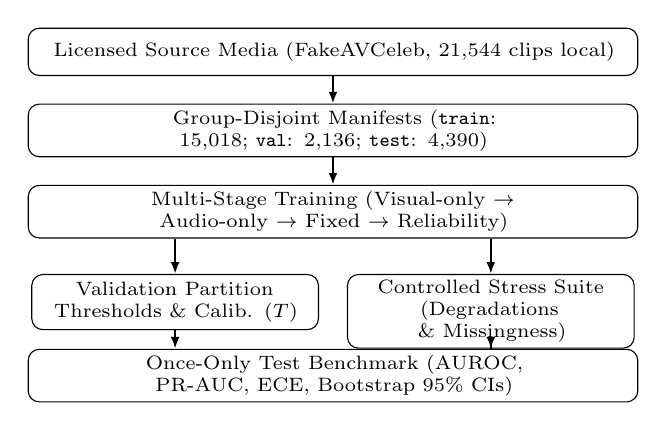
\begin{tikzpicture}[
  font=\scriptsize,
  node distance=3.5mm,
  box/.style={draw,rounded corners,align=center,text width=76mm,minimum height=6mm,inner sep=2pt},
  splitbox/.style={draw,rounded corners,align=center,text width=35mm,minimum height=7mm,inner sep=2pt},
  flow/.style={-{Latex[length=1.5mm]},thick}
]
\node[box] (source) {Licensed Source Media (FakeAVCeleb, 21,544 clips local)};
\node[box,below=of source] (manifest) {Group-Disjoint Manifests (\texttt{train}: 15,018; \texttt{val}: 2,136; \texttt{test}: 4,390)};
\node[box,below=of manifest] (train) {Multi-Stage Training (Visual-only $\to$ Audio-only $\to$ Fixed $\to$ Reliability)};
\node[splitbox,below left=4.5mm and -37mm of train] (val) {Validation Partition\\Thresholds \& Calib. ($T$)};
\node[splitbox,below right=4.5mm and -37mm of train] (stress) {Controlled Stress Suite\\(Degradations \& Missingness)};
\node[box,below=14mm of train] (test) {Once-Only Test Benchmark (AUROC, PR-AUC, ECE, Bootstrap 95\% CIs)};
\draw[flow] (source) -- (manifest);
\draw[flow] (manifest) -- (train);
\draw[flow] (train.south -| val.north) -- (val.north);
\draw[flow] (train.south -| stress.north) -- (stress.north);
\draw[flow] (val.south) -- (val.south |- test.north);
\draw[flow] (stress.south) -- (stress.south |- test.north);
\end{tikzpicture}
\caption{Planned experimental evaluation and leakage-control pipeline. Validation supports model selection and calibration; the test partition is evaluated once.}
\label{fig:protocol}
\end{figure}

\subsection{Baseline Ladder and Stress Testing Suite}
To verify the contribution of each component, we establish a strict baseline hierarchy: (1) Visual-only encoder; (2) Audio-only encoder; (3) Late equal-logit averaging; (4) Feature concatenation + MLP; (5) Fixed learned global weights ($w_v, w_a = \text{const}$); (6) Reliability fusion without synchronization ($c=0$); (7) Reliability fusion without quality features ($q_v, q_a = 0$); and (8) Full proposed reliability-aware system.

The robustness stress suite assesses performance under controlled perturbations:
\begin{itemize}
    \item \textbf{Visual Degradations:} H.264 video compression at Constant Rate Factors (CRF) 18, 28, and 38; spatial downsampling to 720p, 480p, and 360p; Gaussian blur ($\sigma \in \{1, 2, 3\}$); and frame drop (25\%, 50\%).
    \item \textbf{Audio Degradations:} Additive White Gaussian Noise (AWGN) at 20, 10, and 0 dB SNR; MP3 and AAC compression (64, 32 kbps); low-pass filtering (3 kHz cutoff); and packet-loss dropout, following ASVspoof 2021 protocols~\cite{liu2023asvspoof}.
    \item \textbf{Missing Modalities:} Complete audio muting ($m_a=1$) and face occlusion ($m_v=1$), testing whether the gate smoothly shifts $w_m \to 0$ without catastrophic failure, as formulated by Cai et al.~\cite{cai2025modality}.
\end{itemize}

\section{Preliminary Results and Result Analysis}

\subsection{Data-Pipeline Verification Status}
The team reports that the master source table and identity-disjoint split manifests have been generated from the local FakeAVCeleb copy. The inventory contains 21,544 clips, partitioned into 15,018 training, 2,136 validation and 4,390 test clips (69.7\%, 9.9\% and 20.4\%). The pipeline verification report states zero identity overlap and 67 passing unit tests, including checks for split exclusivity, duplicate hashes, missing-modality masking and gate weights summing to one. These are reported pipeline results, not test-set model metrics.

The published FakeAVCeleb table is strongly imbalanced (500 real and 19,500 fake clips)~\cite{khalid2021}, while the local audit inventories 21,544 clips. The local split class composition should therefore be stated separately. Class-balanced sampling, AUROC, PR-AUC and balanced accuracy are used because accuracy alone can be misleading under imbalance.

\begin{table}[t]
\caption{Identity-disjoint split sizes and intended use.}
\label{tab:splits}
\centering
\scriptsize
\setlength{\tabcolsep}{3pt}
\begin{tabular}{lrr}
\toprule
\textbf{Partition} & \textbf{Clips} & \textbf{Share} \\
\midrule
Training & 15,018 & 69.7\% \\
Validation & 2,136 & 9.9\% \\
Test & 4,390 & 20.4\% \\
Total & 21,544 & 100\% \\
\bottomrule
\end{tabular}
\end{table}

\subsection{One-Epoch Validation Snapshot}
Table~\ref{tab:preliminary} gives the validation AUROC recorded after the first epoch. Values are preliminary and validation-only.

\begin{table}[t]
\caption{One-Epoch Validation AUROC and Model Comparison}
\label{tab:preliminary}
\centering
\scriptsize
\setlength{\tabcolsep}{2.5pt}
\begin{tabular}{lccccc}
\toprule
\textbf{Model Variant} & \textbf{AUROC} & \textbf{Rank} & $\Delta_{\mathrm{audio}}$ & $\Delta_{\mathrm{visual}}$ & $\Delta_{\mathrm{fixed}}$ \\
\midrule
Visual-only baseline & 0.7974 & 3 & $-0.0651$ & --- & $-0.1452$ \\
Audio-only baseline & 0.8625 & 2 & --- & $+0.0651$ & $-0.0801$ \\
Equal-weight fixed & \textbf{0.9426} & 1 & $+0.0801$ & $+0.1452$ & --- \\
Reliability-aware & 0.7957 & 4 & $-0.0668$ & $-0.0017$ & $-0.1469$ \\
\bottomrule
\end{tabular}
\end{table}

\subsection{Technical and Forensic Analysis of Validation Results}
Equal-weight fusion exceeds the stronger unimodal branch, audio-only, by 0.0801 AUROC and visual-only by 0.1452. The audio branch is 0.0651 above the visual branch after one epoch; this early difference does not establish their final ranking. Reliability-aware fusion trails fixed fusion by 0.1469 and audio-only by 0.0668. Its 0.0017 difference from visual-only should not be interpreted without uncertainty estimates. The fixed-fusion value satisfies the numerical comparison for proceeding to gate evaluation in this snapshot, but does not establish reproducibility or final performance.

On clean validation clips, both streams may provide complementary evidence, and equal weighting can combine them without learning a routing function~\cite{zhou2021}. This is not a general guarantee: naive fusion can underperform unimodal models in other settings~\cite{muppalla2023}.

The following explanations for the reliability gate's early deficit are candidates, not tested causes:
\begin{table*}[t]
\caption{Candidate explanations for the early reliability-fusion deficit and diagnostics.}
\label{tab:diagnostics}
\centering
\scriptsize
\setlength{\tabcolsep}{4pt}
\renewcommand{\arraystretch}{1.08}
\begin{tabular}{>{\raggedright\arraybackslash}p{0.20\textwidth}>{\raggedright\arraybackslash}p{0.34\textwidth}>{\raggedright\arraybackslash}p{0.38\textwidth}}
\toprule
\textbf{Candidate explanation} & \textbf{Possible mechanism} & \textbf{Diagnostic} \\
\midrule
Gate cold start & Randomly initialized gate weights may perturb the fused representation early in training. & Log weight distributions and gate entropy; try $\mathcal{L}_{bal}$ ($\eta>0$) during warm-up only. \\
Noisy early soft targets & Uncalibrated unimodal losses may produce noisy targets and the KL term may compete with fused classification. & Sweep $\beta$ and $\tau_r$; delay $\mathcal{L}_{rel}$ until modality heads stabilize. \\
Learning-speed imbalance & Audio and visual branches may learn at different rates~\cite{wang2020gblend,peng2022ogm}. & Plot per-branch loss curves and compare with staged freezing. \\
Joint training from step zero & Encoders, projectors, heads and gate may all change together from the first step. & Freeze encoders for five epochs, then unfreeze the last two blocks. \\
Run-to-run variance & One epoch from one run cannot separate an effect from optimization noise. & Repeat with seeds 42, 123 and 7; report identity-bootstrap intervals. \\
\bottomrule
\end{tabular}
\end{table*}

The gate is intended to be evaluated for resilience when a stream is degraded or missing. The clean-data snapshot does not test that hypothesis. If reliability fusion does not help after warm-up and under degradation, that is a reportable result and the project claim should be adjusted accordingly.

\subsection{Hypothesis Status and Remaining Experiments}
All four project hypotheses remain unevaluated. Table~\ref{tab:hypotheses} states the required evidence.

\begin{table*}[t]
\caption{Hypothesis status and evidence required for evaluation.}
\label{tab:hypotheses}
\centering
\scriptsize
\setlength{\tabcolsep}{3pt}
\renewcommand{\arraystretch}{1.06}
\begin{tabular}{c>{\raggedright\arraybackslash}p{0.34\textwidth}>{\raggedright\arraybackslash}p{0.16\textwidth}>{\raggedright\arraybackslash}p{0.34\textwidth}}
\toprule
\textbf{ID} & \textbf{Hypothesis} & \textbf{Status} & \textbf{Evidence required} \\
\midrule
H1 & Reliability fusion has higher mean AUROC than equal-weight and concatenation fusion on the degradation suite. & Not evaluated; clean snapshot favors fixed fusion. & Mean AUROC over video/audio degradations, three seeds and identity-bootstrap interval for the difference. \\
H2 & Under isolated audio or video degradation, gate weights shift as expected and reduce performance drop versus fixed fusion. & Not evaluated. & Mean $w_v,w_a$ by degradation, correlation with severity and metric drop from clean. \\
H3 & On unseen manipulation categories, the model matches or exceeds the strongest unimodal baseline. & Not evaluated. & Per-family AUROC with 95\% intervals for a family held out before training. \\
H4 & A compact model achieves practical short-window latency with documented accuracy cost. & Not evaluated; some parameter counts are derived. & Parameters, checkpoint size, peak memory and p50/p95 latency on named GPU and CPU. \\
\bottomrule
\end{tabular}
\end{table*}

The planned completion sequence is: (1) full-length unimodal baselines for 30 epochs, early stopping and seeds 42/123/7; (2) fixed-fusion comparisons covering equal-logit averaging, concatenation, learned global weights and equal weights; (3) staged reliability fusion with five frozen epochs and sweeps over $\beta$, $\tau_r$ and $T_g$; (4) ablations without synchronization and quality features; (5) cross-manipulation, degradation and missing-modality evaluation; and (6) validation-only calibration, efficiency profiling and a once-only final test pass.

\section{Limitations and Responsible Use}
Each variant has one recorded epoch and one run, so observed differences cannot be separated from run-to-run variation. Only validation results are available; no test metrics, identity-bootstrap intervals, calibration, degradation, missing-modality or cross-manipulation results have been produced. The available snapshot reports only AUROC; PR-AUC, balanced accuracy, F1, calibration and latency remain to be measured. Saved history files are local derived artifacts excluded from version control, so values should be re-exported from final runs.

This system is an academic research detector and cannot serve as legal or forensic proof of malicious intent. Its predictions may degrade on unseen generative architectures, non-frontal poses or novel accents. All datasets are processed locally in compliance with academic licenses; no biometric data or copyrighted video is redistributed.

\section{Conclusion}
The selected stack addresses aligned audio-video inputs, compact encoders, per-window reliability estimation, leakage-resistant splits and calibrated evaluation. The data pipeline reports identity-disjoint partitions of 15,018, 2,136 and 4,390 clips. In the single-epoch validation snapshot, equal-weight fusion leads with AUROC 0.9426, while reliability-aware fusion records 0.7957. This evidence is preliminary and cannot decide whether reliability gating helps. Repeated seeds, staged training, gate diagnostics, degradation and missing-modality evaluation, cross-manipulation testing, calibration and a once-only final test remain necessary; outcomes will be reported according to those measurements.

\begin{thebibliography}{00}
\balance

\bibitem{haliassos2021}
A.~Haliassos, K.~Vougioukas, S.~Petridis, and M.~Pantic, ``Lips don't lie: A generalisable and robust approach to face forgery detection,'' in \emph{Proc. IEEE/CVF Conf. Comput. Vis. Pattern Recognit. (CVPR)}, 2021, pp. 5039--5049, doi: \href{https://doi.org/10.1109/CVPR46437.2021.00500}{10.1109/CVPR46437.2021.00500}.

\bibitem{liu2023asvspoof}
X.~Liu, X.~Wang, M.~Sahidullah, J.~Patino, H.~Delgado, T.~Kinnunen, M.~Todisco, J.~Yamagishi, N.~Evans, A.~Nautsch, and K.-A. Lee, ``ASVspoof 2021: Towards spoofed and deepfake speech detection in the wild,'' \emph{IEEE/ACM Trans. Audio, Speech, Lang. Process.}, vol.~31, pp. 2507--2522, 2023, doi: \href{https://doi.org/10.1109/TASLP.2023.3285283}{10.1109/TASLP.2023.3285283}.

\bibitem{tak2021rawnet2}
H.~Tak, J.~Patino, M.~Todisco, A.~Nautsch, N.~Evans, and A.~Larcher, ``End-to-end anti-spoofing with RawNet2,'' in \emph{Proc. IEEE Int. Conf. Acoust., Speech Signal Process. (ICASSP)}, 2021, pp. 6369--6373, doi: \href{https://doi.org/10.1109/ICASSP39728.2021.9414234}{10.1109/ICASSP39728.2021.9414234}.

\bibitem{jung2022aasist}
J.-w.~Jung, H.-S.~Heo, H.~Tak, H.-j.~Shim, J.~S.~Chung, B.-J.~Lee, H.-J.~Yu, and N.~Evans, ``AASIST: Audio anti-spoofing using integrated spectro-temporal graph attention networks,'' in \emph{Proc. IEEE Int. Conf. Acoust., Speech Signal Process. (ICASSP)}, 2022, pp. 6367--6371, doi: \href{https://doi.org/10.1109/ICASSP43922.2022.9747766}{10.1109/ICASSP43922.2022.9747766}.

\bibitem{khalid2021}
H.~Khalid, S.~Tariq, M.~Kim, and S.~S.~Woo, ``FakeAVCeleb: A novel audio-video multimodal deepfake dataset,'' in \emph{Proc. Adv. Neural Inf. Process. Syst. (NeurIPS) Datasets and Benchmarks Track}, 2021.

\bibitem{muppalla2023}
S.~Muppalla, S.~Jia, and S.~Lyu, ``Integrating audio-visual features for multimodal deepfake detection,'' in \emph{Proc. IEEE MIT Undergrad. Res. Technol. Conf. (URTC)}, 2023, pp. 1--6, doi: \href{https://doi.org/10.1109/URTC60662.2023.10534969}{10.1109/URTC60662.2023.10534969}.

\bibitem{zhou2021}
Y.~Zhou and S.-N.~Lim, ``Joint audio-visual deepfake detection,'' in \emph{Proc. IEEE/CVF Int. Conf. Comput. Vis. (ICCV)}, 2021, pp. 14800--14809, doi: \href{https://doi.org/10.1109/ICCV48922.2021.01453}{10.1109/ICCV48922.2021.01453}.

\bibitem{cai2025modality}
Y.~Cai, P.~Chen, J.~Tian, J.~Liu, J.~Dai, X.~Wang, Y.~Chai, S.~Jia, S.~Lyu, and J.~Han, ``Modality-agnostic deepfakes detection,'' in \emph{Proc. ACM Workshop Inf. Hiding Multimedia Security (IH\&MMSec)}, 2025, doi: \href{https://doi.org/10.1145/3733102.3733133}{10.1145/3733102.3733133}.

\bibitem{chugh2020}
K.~Chugh, P.~Gupta, A.~Dhall, and R.~Subramanian, ``Not made for each other---Audio-visual dissonance-based deepfake detection and localization,'' in \emph{Proc. ACM Int. Conf. Multimedia (MM)}, 2020, pp. 439--447, doi: \href{https://doi.org/10.1145/3394171.3413700}{10.1145/3394171.3413700}.

\bibitem{chung2016}
J.~S.~Chung and A.~Zisserman, ``Out of time: Automated lip sync in the wild,'' in \emph{Proc. Asian Conf. Comput. Vis. (ACCV) Workshops}, LNCS, vol. 10117, Springer, 2017, pp. 251--263, doi: \href{https://doi.org/10.1007/978-3-319-54427-4_19}{10.1007/978-3-319-54427-4\_19}.

\bibitem{wang2024}
R.~Wang, D.~Ye, L.~Tang, Y.~Zhang, and J.~Deng, ``AVT$^{2}$-DWF: Improving deepfake detection with audio-visual fusion and dynamic weighting strategies,'' \emph{IEEE Signal Process. Lett.}, vol.~31, pp. 1960--1964, 2024, doi: \href{https://doi.org/10.1109/LSP.2024.3433596}{10.1109/LSP.2024.3433596}.

\bibitem{mittal2020}
T.~Mittal, U.~Bhattacharya, R.~Chandra, A.~Bera, and D.~Manocha, ``Emotions don't lie: An audio-visual deepfake detection method using affective cues,'' in \emph{Proc. ACM Int. Conf. Multimedia (MM)}, 2020, pp. 2823--2832, doi: \href{https://doi.org/10.1145/3394171.3413570}{10.1145/3394171.3413570}.

\bibitem{dolhansky2020}
B.~Dolhansky, J.~Bitton, B.~Pflaum, J.~Lu, R.~Howes, M.~Wang, and C.~Canton~Ferrer, ``The DeepFake Detection Challenge (DFDC) dataset,'' arXiv:2006.07397, 2020, doi: \href{https://doi.org/10.48550/arXiv.2006.07397}{10.48550/arXiv.2006.07397}.

\bibitem{yang2023}
W.~Yang, X.~Zhou, Z.~Chen, B.~Guo, Z.~Ba, Z.~Xia, X.~Cao, and K.~Ren, ``AVoiD-DF: Audio-visual joint learning for detecting deepfake,'' \emph{IEEE Trans. Inf. Forensics Security}, vol.~18, pp. 2015--2029, 2023, doi: \href{https://doi.org/10.1109/TIFS.2023.3262148}{10.1109/TIFS.2023.3262148}.

\bibitem{oorloff2024}
T.~Oorloff, S.~Koppisetti, N.~Bonettini, D.~Solanki, B.~Colman, Y.~Yacoob, A.~Shahriyari, and G.~Bharaj, ``AVFF: Audio-visual feature fusion for video deepfake detection,'' in \emph{Proc. IEEE/CVF Conf. Comput. Vis. Pattern Recognit. (CVPR)}, 2024, pp. 27102--27112, doi: \href{https://doi.org/10.1109/CVPR52733.2024.02559}{10.1109/CVPR52733.2024.02559}.

\bibitem{ilyas2023}
H.~Ilyas, A.~Javed, and K.~M.~Malik, ``AVFakeNet: A unified end-to-end dense Swin Transformer deep learning model for audio--visual deepfakes detection,'' \emph{Appl. Soft Comput.}, vol. 136, p. 110124, 2023, doi: \href{https://doi.org/10.1016/j.asoc.2023.110124}{10.1016/j.asoc.2023.110124}.

\bibitem{astrid2024}
M.~Astrid, E.~Ghorbel, and D.~Aouada, ``Statistics-aware audio-visual deepfake detector,'' in \emph{Proc. IEEE Int. Conf. Image Process. (ICIP)}, 2024, pp. 2470--2476, doi: \href{https://doi.org/10.1109/ICIP51287.2024.10648224}{10.1109/ICIP51287.2024.10648224}.

\bibitem{wang2020gblend}
W.~Wang, D.~Tran, and M.~Feiszli, ``What makes training multi-modal classification networks hard?,'' in \emph{Proc. IEEE/CVF Conf. Comput. Vis. Pattern Recognit. (CVPR)}, 2020, pp. 12695--12705, doi: \href{https://doi.org/10.1109/CVPR42600.2020.01271}{10.1109/CVPR42600.2020.01271}.

\bibitem{peng2022ogm}
X.~Peng, Y.~Wei, A.~Deng, D.~Wang, and D.~Hu, ``Balanced multimodal learning via on-the-fly gradient modulation,'' in \emph{Proc. IEEE/CVF Conf. Comput. Vis. Pattern Recognit. (CVPR)}, 2022, pp. 8238--8247, doi: \href{https://doi.org/10.1109/CVPR52688.2022.00806}{10.1109/CVPR52688.2022.00806}.

\bibitem{terhorst2020serfiq}
P.~Terh{\"o}rst, J.~N.~Kolf, N.~Damer, F.~Kirchbuchner, and A.~Kuijper, ``SER-FIQ: Unsupervised estimation of face image quality based on stochastic embedding robustness,'' in \emph{Proc. IEEE/CVF Conf. Comput. Vis. Pattern Recognit. (CVPR)}, 2020, pp. 5650--5659, doi: \href{https://doi.org/10.1109/CVPR42600.2020.00569}{10.1109/CVPR42600.2020.00569}.

\bibitem{paszke2019}
A.~Paszke et al., ``PyTorch: An imperative style, high-performance deep learning library,'' in \emph{Proc. Adv. Neural Inf. Process. Syst. (NeurIPS)}, 2019, pp. 8024--8035.

\bibitem{viola2001}
P.~Viola and M.~Jones, ``Rapid object detection using a boosted cascade of simple features,'' in \emph{Proc. IEEE Comput. Soc. Conf. Comput. Vis. Pattern Recognit. (CVPR)}, 2001, pp. I-511--I-518.

\bibitem{howard2019}
A.~Howard et al., ``Searching for MobileNetV3,'' in \emph{Proc. IEEE/CVF Int. Conf. Comput. Vis. (ICCV)}, 2019, pp. 1314--1324.

\bibitem{loschilov2019}
I.~Loshchilov and F.~Hutter, ``Decoupled weight decay regularization,'' in \emph{Proc. Int. Conf. Learn. Represent. (ICLR)}, 2019.

\bibitem{loschilov2017}
I.~Loshchilov and F.~Hutter, ``SGDR: Stochastic gradient descent with warm restarts,'' in \emph{Proc. Int. Conf. Learn. Represent. (ICLR)}, 2017.

\bibitem{micikevicius2018}
P.~Micikevicius et al., ``Mixed precision training,'' in \emph{Proc. Int. Conf. Learn. Represent. (ICLR)}, 2018.

\bibitem{pedregosa2011}
F.~Pedregosa et al., ``Scikit-learn: Machine learning in Python,'' \emph{J. Mach. Learn. Res.}, vol.~12, pp. 2825--2830, 2011.

\bibitem{guo2017}
C.~Guo, G.~Pleiss, Y.~Sun, and K.~Q. Weinberger, ``On calibration of modern neural networks,'' in \emph{Proc. Int. Conf. Mach. Learn. (ICML)}, PMLR, vol.~70, 2017, pp. 1321--1330.

\bibitem{oord2018}
A.~van den Oord, Y.~Li, and O.~Vinyals, ``Representation learning with contrastive predictive coding,'' arXiv:1807.03748, 2018.

\end{thebibliography}

\end{document}
